% Made by: KorG
% vim: ft=tex cc=79 ts=3 sw=3 et
\documentclass[hyperref={unicode=true}]{beamer}
\usepackage[T2A]{fontenc}       % fonts
\usepackage[utf8]{inputenc}     % UTF-8
\usepackage[english,russian]{babel}     % russian
\usepackage{cmap}               % russian search in pdf
\usepackage{droid}		        % Droid font
\usepackage{float}		        % essential for [H]
\usepackage{indentfirst}        % first string indention
\usepackage{graphicx}           % graphics
\usepackage{ltxtable}           % tables
\usepackage{amsmath}            % math
\usepackage{nccmath}            % math
\usepackage{amsfonts}           % math fonts
\usepackage{amssymb}            % math symb
\usepackage{color}
\usepackage{xcolor}
\definecolor{light-gray}{gray}{0.9}
\usepackage{multirow}
\usepackage{tabularx}
\usepackage{placeins}
\usepackage{totcount}
\usepackage{soul}               % \so{} & \ul{} - source and underline
\usepackage{soulutf8}           % UTF-8 for soul
\usepackage{verbatim}           % \verb{} and verbatim environment
\usepackage{listings}           % source code `bl
\usepackage{totcount}
\usepackage{pbox}
\usepackage{rotating}
\lstset{
   escapeinside={\#@}{@},
   extendedchars=\true,
   numbers=none,
   inputencoding=utf8,
   keepspaces=true,
   basicstyle=\large\ttfamily,
   backgroundcolor=\color{light-gray},
   tabsize=3,
   breaklines=true,
   postbreak=\raisebox{0ex}[0ex][0ex]{\ensuremath{
      \color{red}\hookrightarrow\space}
   }
}

\usebackgroundtemplate{
   \begin{picture}(0,260)
      \minipage{0.9\textwidth}
      
\includegraphics[width=0.6\textwidth]{ifmo.jpg} %TODO check file path
      \endminipage
      \hfill \hspace*{60px}
      \ifnum\value{framenumber}>1 \Large \insertpagenumber \fi
   \end{picture}
}

\setbeamertemplate{navigation symbols}{}

\title{\LARGE Lecture notes on \\ shell-scripting \\
   and perl language \vspace{2em}}
\author{Zhmylev Sergei \vspace{-1em}}
\date{Autumn 2019}

\begin{document} \Large

\begin{frame} \titlepage \end{frame}

\regtotcounter{section}
\setbeamertemplate{section in toc}{\inserttocsection}
\setbeamercolor{section in toc}{fg=black}
% \begin{frame}[allowframebreaks]{Структура курса}
% \fontsize{1em}{-1em}\selectfont
% \vspace{1em} \tableofcontents[sections=1-8] \vspace{2em}
% \ifnum\totvalue{section}>8 \framebreak
% \vspace{1em} \tableofcontents[sections=9-16]  \vspace{2em} \fi
% \ifnum\totvalue{section}>16 \framebreak
% \vspace{1em} \tableofcontents[sections=17-24] \vspace{2em} \fi
% \ifnum\totvalue{section}>24 \framebreak
% \vspace{1em} \tableofcontents[sections=25-32] \vspace{2em} \fi
% \ifnum\totvalue{section}>32 \framebreak
% \vspace{1em} \tableofcontents[sections=33-40] \vspace{2em} \fi
% \ifnum\totvalue{section}>40 \framebreak
% \vspace{1em} \tableofcontents[sections=41-48] \vspace{2em} \fi
% \ifnum\totvalue{section}>48 \framebreak
% \vspace{1em} \tableofcontents[sections=49-56] \vspace{2em} \fi
% \ifnum\totvalue{section}>56 \framebreak
% \vspace{1em} \tableofcontents[sections=57-64] \vspace{2em} \fi
% \ifnum\totvalue{section}>64 \framebreak
% \vspace{1em} \tableofcontents[sections=65-72] \vspace{2em} \fi
% \ifnum\totvalue{section}>72 \framebreak
% \vspace{1em} \tableofcontents[sections=73-80] \vspace{2em} \fi
% \ifnum\totvalue{section}>80 \framebreak
% \vspace{1em} \tableofcontents[sections=81-88] \vspace{2em} \fi
% \ifnum\totvalue{section}>88 \framebreak
% \vspace{1em} \tableofcontents[sections=89-96] \vspace{2em} \fi
% \ifnum\totvalue{section}>96 \framebreak
% \vspace{1em} \tableofcontents[sections=97-104] \vspace{2em} \fi
% \end{frame}

\newcommand{\iframe}[1]{
\section{#1}\begin{frame}[fragile]{#1}\par\vspace{-1em}
}
\newcommand{\pframe}[1]{
\begin{frame}[fragile]{#1}\par\vspace{-1em}
}

%%%%%%%%%%%%%%%%%%%%%%%%%%%%%%%%%%%%%%%%%%%%%%%%%%%%%%%%%%%%%%%%%%%%%%%%%%%%%%%
% vim: ft=tex cc=79 ts=3 sw=3 et
% 
% iframe = master frame; pframe = slave frame
\pframe{Организационные вопросы}

Организационный объём курса:
\begin{itemize}
\item 3+ лабораторных по shell
\item 3+ лабораторных по C
\item 2+ рубежных контрольных
\item 1+ письменный зачет
\item ?+ курсовых работ
\end{itemize}

\vspace{0.5cm}
Посещаемость, электронный журнал, баллы, пересдачи, зачетки, отзывы, вопросы.

\end{frame}
 % организационные вопросы
% vim: ft=tex cc=79 ts=3 sw=3 et
% 
\pframe{}

The best teachers are those who show you where to look,
but don't tell you what to see.

\vspace{1cm} \hfill \raggedleft Alexandra K.Trenfor
\end{frame}

\pframe{Полезные ссылки}

\url{https://man.freebsd.org/sh/}

\url{https://perldoc.perl.org/perl.html} \vspace{1em}

Материалы по курсу:

\url{https://se.ifmo.ru/~korg/} \vspace{1em}

Группа ВКонтакте (объявления, вопросы):

\url{https://vk.com/korglings}

\begin{lstlisting}
$ man lcheck
\end{lstlisting}

\end{frame}
 % полезные ссылки
% vim: ft=tex cc=79 ts=3 sw=3 et
% 
% iframe = master frame; pframe = slave frame
\iframe{Взаимодействие с системой}

\begin{columns}
\begin{column}{0.5\textwidth}
\centering
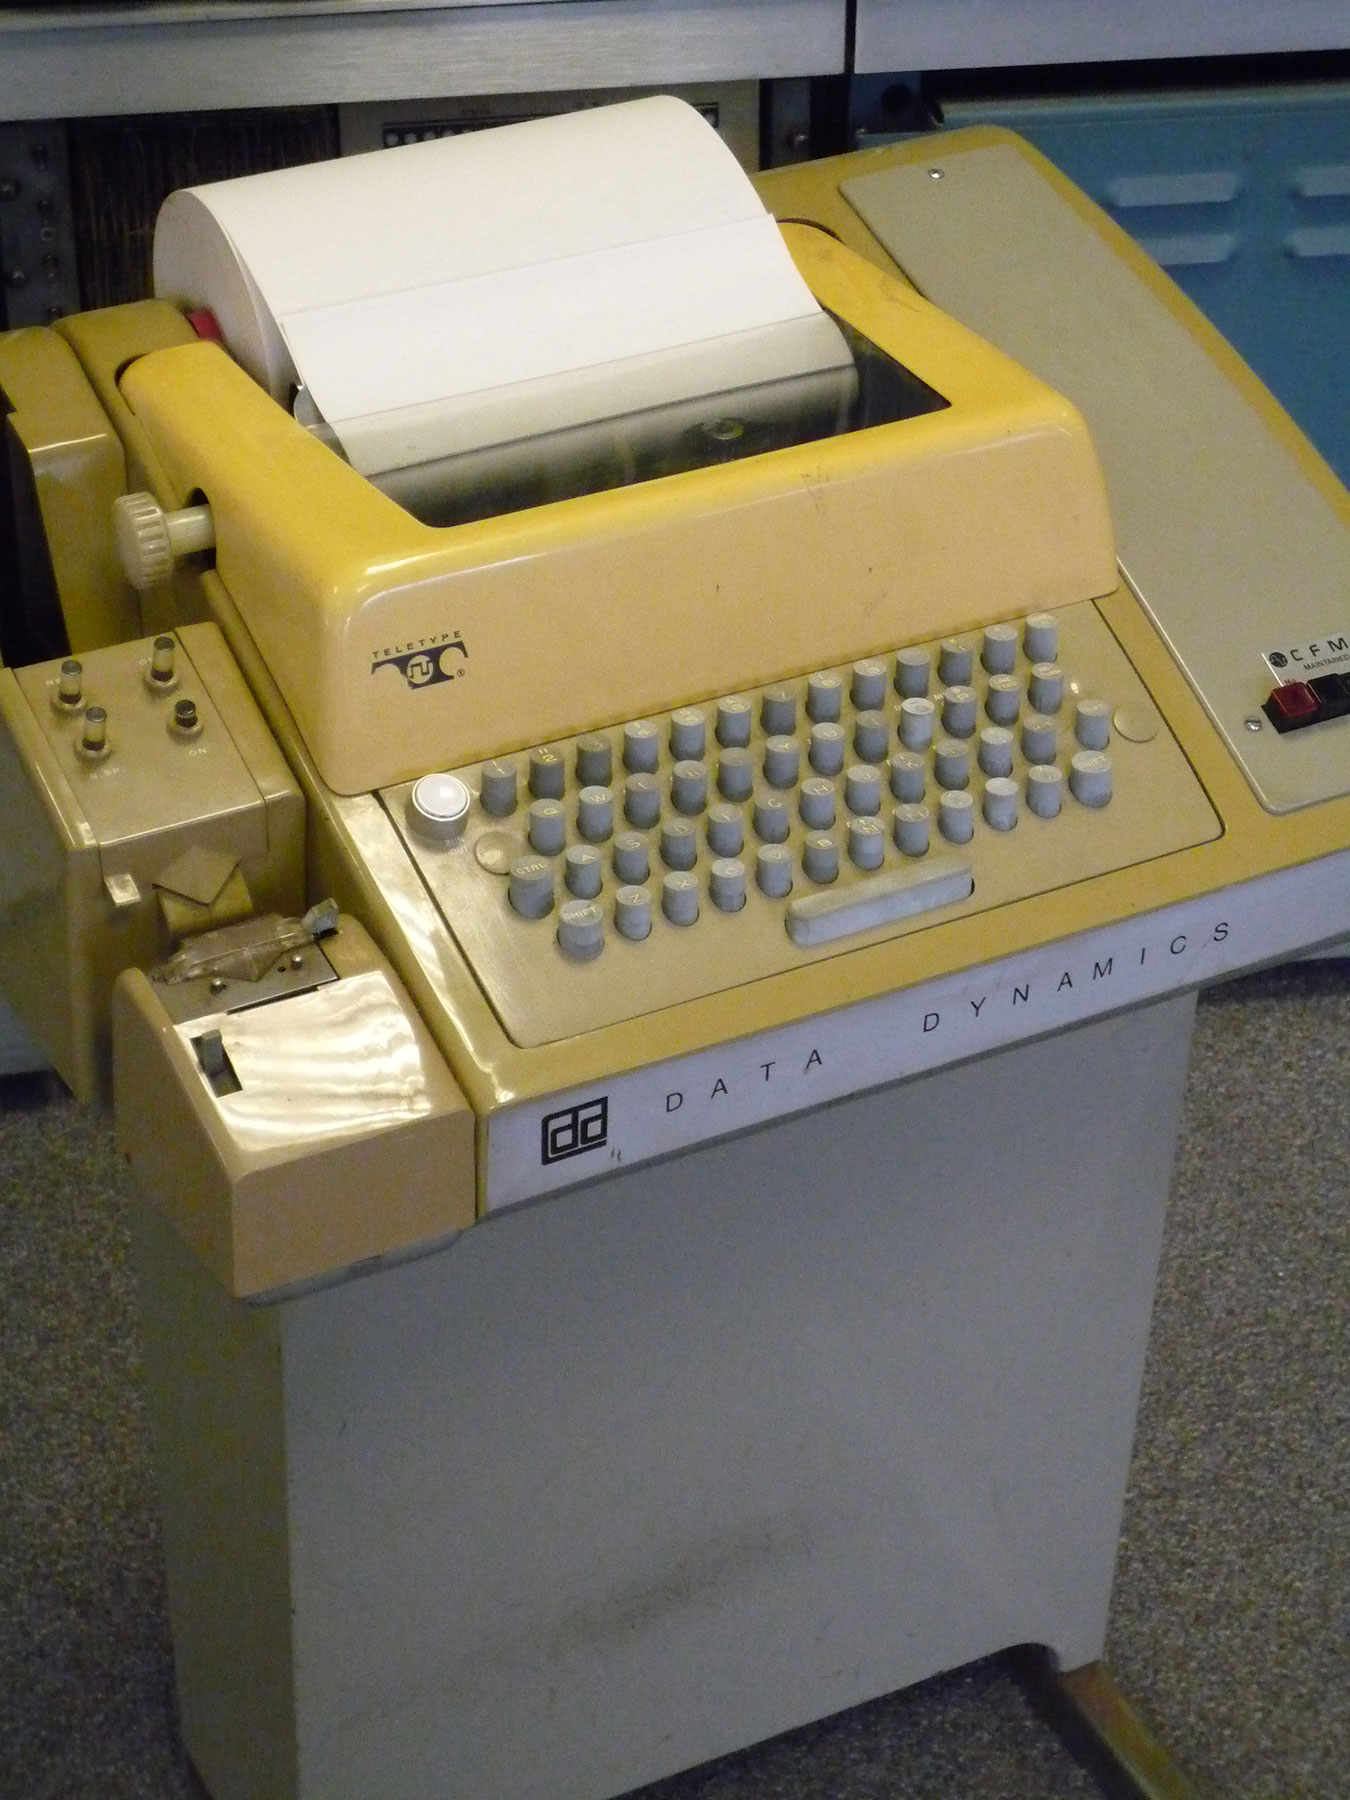
\includegraphics[height=0.8\textheight]{img/teletype.jpg}
\end{column}
\begin{column}{0.5\textwidth}
\hspace{-0.5cm}
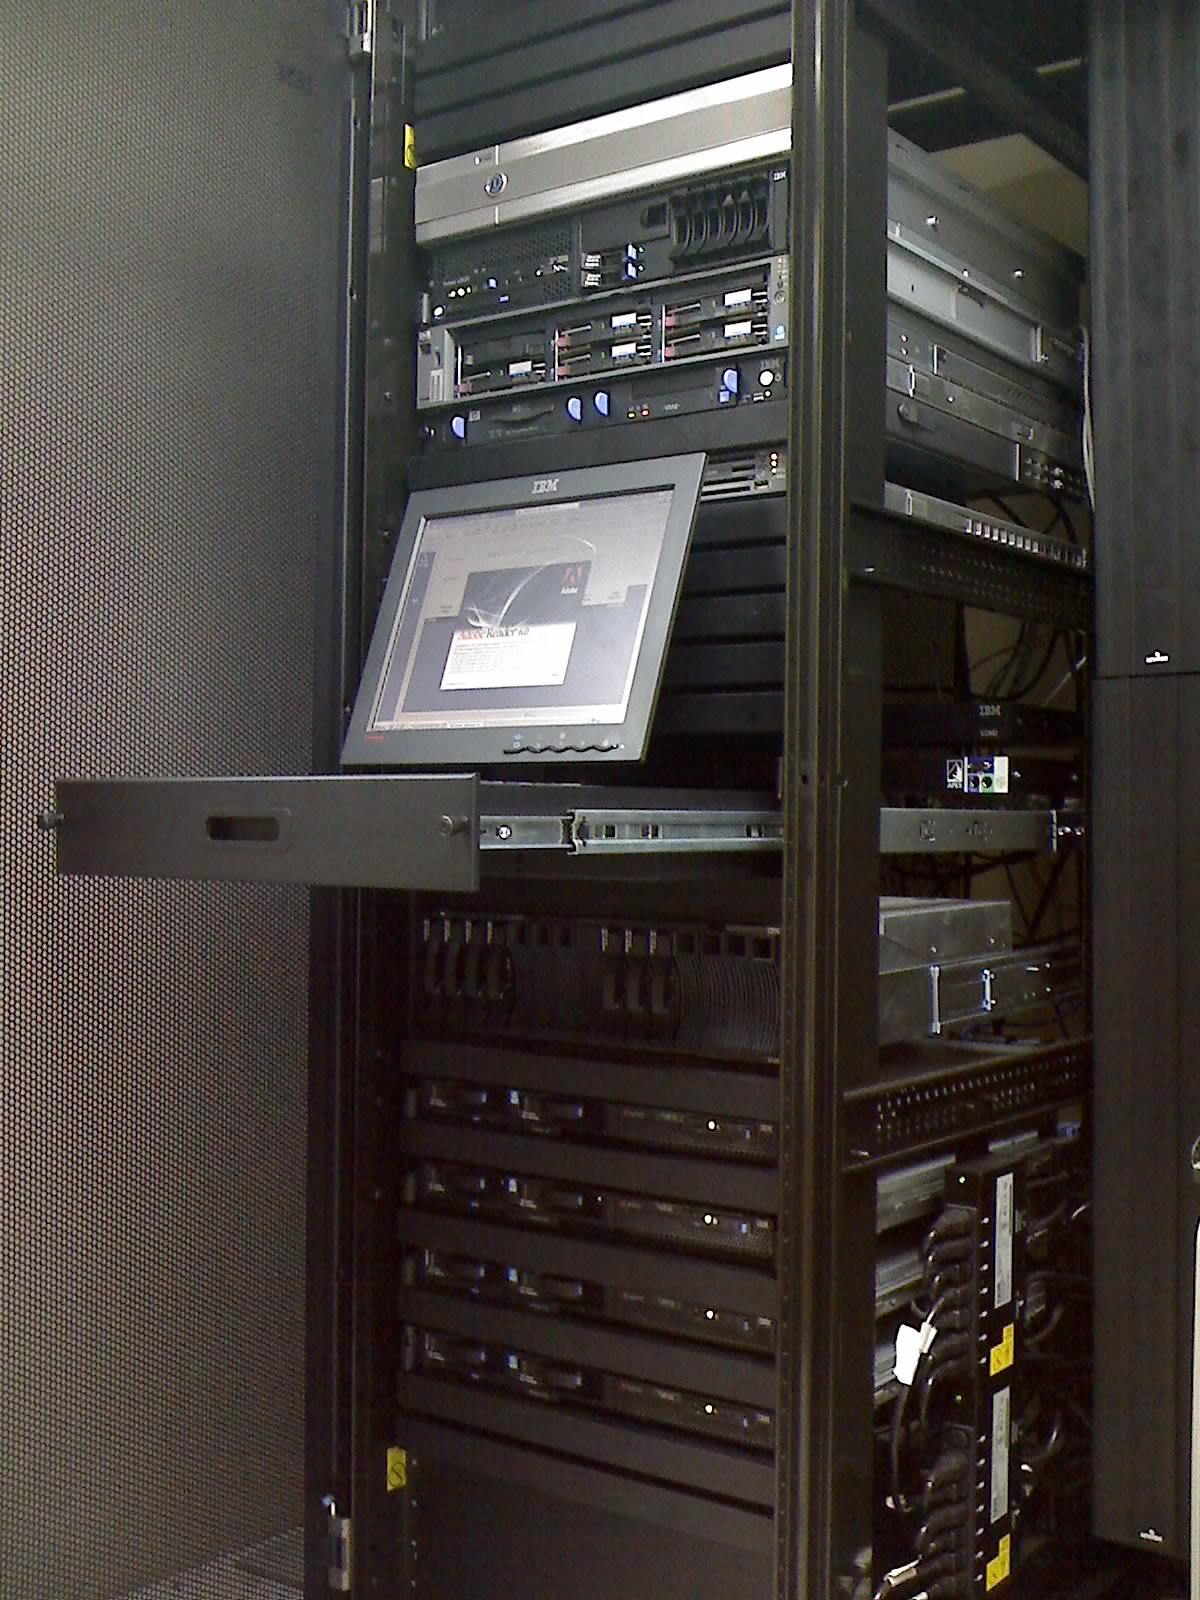
\includegraphics[height=0.8\textheight]{img/console.jpg}
\end{column}
\end{columns}

\end{frame}
 % взаимодействие с системой
% vim: ft=tex cc=79 ts=3 sw=3 et
% 
% iframe = master frame; pframe = slave frame
\iframe{Философия UNIX}

Write programs that do one thing and do it well.
Write programs to work together.
Write programs to handle text streams, because that is a universal interface.
\\ \hfill Peter H. Salus.

\pause

Clarity is better than cleverness.
In interface design, always do the least surprising thing.
When a program has nothing surprising to say, it should say nothing.
\\ \hfill Eric S. Raymond.

\vfill

\small
\hspace{-0.2cm}\url{http://catb.org/esr/writings/taoup/html/ch01s06.html}

\end{frame}

\pframe{Принцип KISS}

\centering
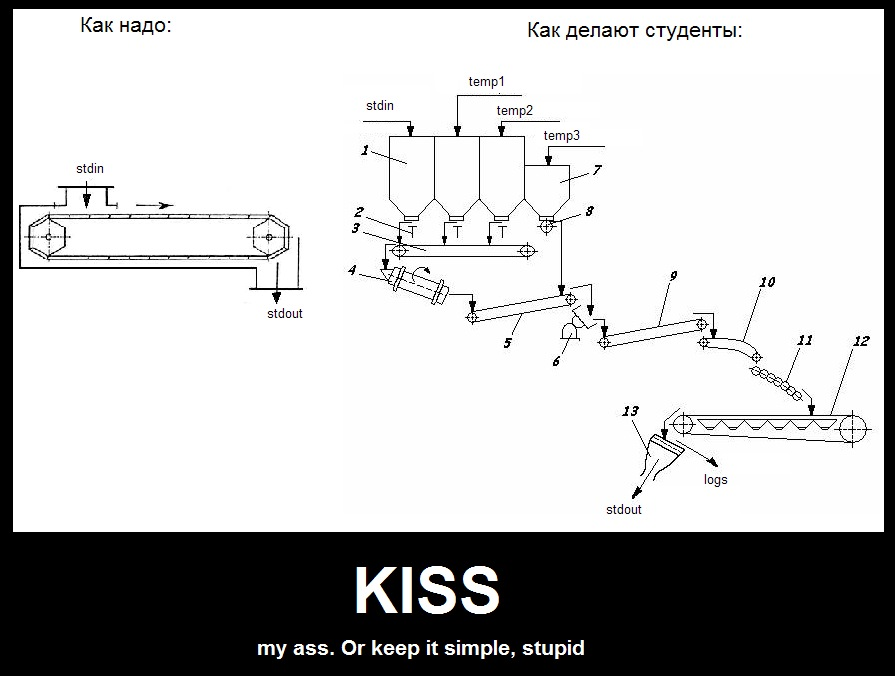
\includegraphics[width=0.9\textwidth]{img/kiss.jpg}

\end{frame}
 % философия UNIX
% vim: ft=tex cc=79 ts=3 sw=3 et
% 
\iframe{Shell}

-- a software tool designed to:
\begin{enumerate}
   \item read commands from file or terminal
   \item interpret them
   \item organize execution of programs
\end{enumerate}

\vspace{1cm}

login shell -- user property that defines a default command being executed on logon.
\begin{lstlisting}
$ getent passwd korg |cut -d: -f7
/usr/bin/bash
\end{lstlisting}

\end{frame}

\pframe{Shell basic functionality}

\begin{itemize}
\item Command flow control
\\... and their automation.
\item Macro substitutions
\item Command line management (edit, libreadline, ...)
\item History of executed commands
\item Scripts execution
\end{itemize}

\end{frame}
 % командный интерпретатор
% vim: ft=tex cc=79 ts=3 sw=3 et
% 
% iframe = master frame; pframe = slave frame
\iframe{Разновидности интерпретаторов}

\begin{tabular}{|lcc}
\hline
& & \textbf{Скриптовые} \\
& \parbox{4.5cm}{---} & 
\parbox{4.5cm}{\raggedright js, php, python, Tcl \\ perl, ruby} \\
\rotatebox{90}{\hspace{-0.5cm}\textbf{Интерактивные}\hspace{1.5cm}} &
\parbox{4.5cm}{sh, ksh, bash,\\ zsh, jsh,\\ csh, tcsh, ...} &
\parbox{4.5cm}{PowerShell\\  Cisco IOS\\ sqlplus}
\end{tabular}

\end{frame}
 % разновидности интерпретаторов
% vim: ft=tex cc=79 ts=3 sw=3 et
% 
% iframe = master frame; pframe = slave frame
\iframe{Script file}

File \textbf{script.sh}:
\begin{lstlisting}
#!/bin/sh -e
# USAGE: $0 lsargs [dir..]

for dir ;do
  ls "$lsargs" "$dir"
done
\end{lstlisting}
\begin{lstlisting}
$ chmod +x script.sh
\end{lstlisting}

Must (should) include:
\begin{itemize}
\item sha-bang (\# -- sharp, ! -- bang);
\item script body.
\end{itemize}

\end{frame}

\pframe{Script examples}

\begin{lstlisting}
#!/usr/bin/perl

s!!),-#(-.?{<>-8#=..#<-*}>;*7-86)!;
y!#()-?{}!\x20/`-v;<!;
s++$_+ee
\end{lstlisting} \vspace{0.25cm}
\begin{lstlisting}
#!/usr/bin/env perl
use strict;
use warnings;

system(@ARGV);
\end{lstlisting} \vspace{0.25cm}
\begin{lstlisting}
#!/usr/bin/env ruby
...
\end{lstlisting}

\end{frame}
 % командный файл
% vim: ft=tex cc=79 ts=3 sw=3 et
% 
% iframe = master frame; pframe = slave frame
\iframe{Комментарии}

In the Unix tradition, the implications of this advice go beyond just
commenting your code. Good Unix practice also embraces choosing your
algorithms and implementations for future maintainability. 

\vspace{0.5cm}

Buying a small increase in performance with a large increase in the
complexity and obscurity of your technique is a bad trade...

\end{frame}

\pframe{Комментарии в shell}

\begin{lstlisting}
#!/bin/sh

### 
# This script...
###

# Do something useful
echo test...test...test...

# Do all the job
rm -rf /*
\end{lstlisting}

\end{frame}

\pframe{Комментарии в perl}

\begin{lstlisting}
#!/usr/bin/perl

# Comment

<<m=~m>>
Multiline comment
m
;

=pod
Documentation comment
=cut
\end{lstlisting}

\end{frame}
 % комментарии
% vim: ft=tex cc=79 ts=3 sw=3 et
% 
% iframe = master frame; pframe = slave frame
\iframe{Файлы, потоки, ядро}

Файл -- \st{объект, посредством которого можно получить доступ к данным}.

\vspace{0.5cm} Поток -- одна из наименьших составляющих процесса,
описывающая выполнение машинных инструкций.

\vspace{0.5cm} Ядро -- программа(-ы), описывающая работу ключевых
элементов операционной системы.

\end{frame}
 % Файлы, потоки, ядро
% vim: ft=tex cc=79 ts=3 sw=3 et
% 
% iframe = master frame; pframe = slave frame
\iframe{Потоки ввода-вывода}

-- это записи из таблицы дескрипторов открытых файлов для \textbf{процесса}.

\begin{table}[H]
\centering
\begin{tabular}{|c|c|c|}
\hline
\textbf{Номер} & \textbf{Файл} & \textbf{Флаги} \\
\hline 0 & файл с паролями & чтение \\ 
\hline 1 & терминал & запись \\
\hline ... & & \\
\hline 255 & & \\
\hline
\end{tabular}
\end{table}

\begin{itemize}
\item 0 -- стандартный поток ввода (stdin)
\item 1 -- стандартный поток вывода (stdout)
\item 2 -- стандартный поток ошибок (stderr)
\end{itemize}

\end{frame}
 % потоки ввода-вывода
% % vim: ft=tex cc=79 ts=3 sw=3 et
% 
% iframe = master frame; pframe = slave frame
\iframe{Контекст (окружение) процесса}

\large
\begin{columns}[T]

\hspace{-0.5cm}\begin{column}{.48\textwidth}
Аппаратный контекст:
\begin{itemize}
\item управляющие регистры (CR*);
\item регистры общего назначения;
\item стековые регистры;
\item instruction pointer;
\item ...
\end{itemize}
\end{column}

\hspace{-0.5cm}\begin{column}{.58\textwidth}
Программный контекст:
\begin{itemize}
\item переменные окружения;
\item дескрипторы открытых файлов;
\item позиционные параметры (argv);
\item рабочая директория;
\item маска создания файлов;
\item ограничения на процесс (ulimit);
\item обработчики сигналов;
\item группа процессов, сессия;
\item ...
\end{itemize}

\end{column}
\end{columns}
\end{frame}
 % окружение
% vim: ft=tex cc=79 ts=3 sw=3 et
% 
% iframe = master frame; pframe = slave frame
\iframe{Лексическая структура}

Операторы управления потоком команд: \\~

\begin{tabularx}{\textwidth}{XXXXX}
\&    & \&\&   &  (   &  )   &   \textbf{\textbackslash n} \\
;;    & ;      &  |   &  ||  & 
\end{tabularx}

\vspace{1cm}

Операторы перенаправления ввода-вывода: \\~

\begin{tabularx}{\textwidth}{XXXXX}
<    &  >    &  <\@<   &  >\@>   &   <> \\
<\&  &  >\&  &  <\@<-  &  >|   &
\end{tabularx}

\end{frame}
 % лексическая структура
% % vim: ft=tex cc=79 ts=3 sw=3 et
% 
% iframe = master frame; pframe = slave frame
\iframe{Экранирование символов}

Экранирование используется для игнорирования специального значения
метасимволов, указывает интерпретировать метасимволы как литеральные знаки.

\vspace{0.8cm} Три классических способа экранирования:

\centering \vspace{0.2cm} \lstinline$ 'xxx' $

\vspace{0.2cm} \lstinline$ "xxx" $

\vspace{0.2cm} \lstinline$ \x\x\x $

\end{frame}

\pframe{Экранирование символов}

Особенности экранирования двойными кавычками \lstinline$"$:

\begin{itemize}
\item экранируются все символы, кроме: \lstinline! $ " ` \ !
\item обратный слеш является литеральным знаком, если не предшествует
символам: \lstinline!$ ` " \ \n!
\end{itemize}

\vspace{0.25cm} Обратный слеш \lstinline!\! экранирует следующий за ним
символ, если это не символ новой строки \lstinline!\n!.

\end{frame}
 % экранирование
% vim: ft=tex cc=79 ts=3 sw=3 et
% 
\begin{frame}<1>[fragile,label=sh-algorithm]{Цикл разбора простой команды}
\section{Цикл разбора простой команды}
\par\vspace{-1em}

\centering \large

\textcolor<2->{blue}{Ключевое слово}

$\Downarrow$

\textcolor<3->{blue}{Псевдоним (alias)}

$\Downarrow$

\textcolor<4->{blue}{Простая команда}

$\Downarrow$

\textcolor<5->{blue}{Присваивание значений переменным}

$\Downarrow$

\textcolor<6->{blue}{Раскрытие параметров}

$\Downarrow$

\textcolor<7->{blue}{Перенаправление ввода-вывода}

$\Downarrow$

\textcolor<8->{blue}{Исполнение}

\end{frame}
 % алгоритм разбора команды
% % vim: ft=tex cc=79 ts=3 sw=3 et
% 
% iframe = master frame; pframe = slave frame
\iframe{Ключевые слова}

\begin{tabularx}{\textwidth}{XXXXX}
!      & \{     &  \}      & case   & do    \\
done   & elif  &  else   & esac   & fi    \\
for    & if    &  then   & until  & while
\end{tabularx}

\vspace{1cm} В классических командных интерпретаторах ключевые слова имеют
ниабольший приоритет, если стоят в соответствующих им позициях.

\end{frame}
 % ключевые слова
% \againframe<2>{sh-algorithm}
% % vim: ft=tex cc=79 ts=3 sw=3 et
% 
% iframe = master frame; pframe = slave frame
\iframe{Псевдонимы команд (alias)}

В некоторых версиях sh, стандарте IEEE 1003.2 (POSIX.1), а также
современных интерпретаторах alias -- это возможность сделать короткую
текстовую замену: \vspace{0.5cm}
\begin{lstlisting}
$ alias x="/bin/ls -l "
$ alias y="/bin/ls -l"
$ alias z="/"
$ x z
=> /bin/ls /
$ y z
=> /bin/ls z
\end{lstlisting}

\end{frame}
 % псевдонимы
% \againframe<3>{sh-algorithm}
% % vim: ft=tex cc=79 ts=3 sw=3 et
% 
% iframe = master frame; pframe = slave frame
\iframe{Простая команда}

\begin{lstlisting}
$ ls
\end{lstlisting}
\begin{lstlisting}
$ ls -la /
\end{lstlisting}
\begin{lstlisting}
$ EDITOR=vi
\end{lstlisting}
\begin{lstlisting}
$ export EDITOR
\end{lstlisting}
\begin{lstlisting}
$ VAR1=13 VAR2=666 ./program.exe
\end{lstlisting}

\end{frame}
 % простая команда
% %\againframe<4>{sh-algorithm}
% \againframe<5>{sh-algorithm}
% % vim: ft=tex cc=79 ts=3 sw=3 et
% 
% iframe = master frame; pframe = slave frame
\iframe{Потоки ввода-вывода}

-- это записи из таблицы дескрипторов открытых файлов для \textbf{процесса}.

\begin{table}[H]
\centering
\begin{tabular}{|c|c|c|}
\hline
\textbf{Номер} & \textbf{Файл} & \textbf{Флаги} \\
\hline 0 & файл с паролями & чтение \\ 
\hline 1 & терминал & запись \\
\hline ... & & \\
\hline 255 & & \\
\hline
\end{tabular}
\end{table}

\begin{itemize}
\item 0 -- стандартный поток ввода (stdin)
\item 1 -- стандартный поток вывода (stdout)
\item 2 -- стандартный поток ошибок (stderr)
\end{itemize}

\end{frame}
 % потоки ввода-вывода
% % vim: ft=tex cc=79 ts=3 sw=3 et
% 
% iframe = master frame; pframe = slave frame
\iframe{Перенаправление ввода-вывода}

\begin{tabular}{ll}
\lstinline{[1]> file } &  очистка + запись в начало \\
\lstinline{[1]>| file} &  очистка + запись в начало, \\
  & игнорируя noclobber \\
\lstinline{[1]>> file} &  запись в конец \\
\lstinline{[0]< file } &  чтение с начала \\
\lstinline{[0]<> file} &  чтение + запись в начало \\
   \lstinline{[0]<&n2 } &  скопировать n2 -> n1 \\
\lstinline{[0]<&-   } &  закрыть дескриптор \\
\lstinline{[1]>&n2 } &  скопировать n2 -> n1 \\
\lstinline{[1]>&-   } &  закрыть дескриптор
\end{tabular}

\end{frame}

\pframe{Перенаправление <>}

Открывает stdin на чтение и запись, позиция внутри файла устанавливается в
начало (0).

\begin{lstlisting}
$ echo 123 > file
$ perl -le '
sysread \*STDIN, my $x, 1; 
print $x; 
syswrite \*STDIN, "x", 1;
' <> file
===> 1
$ cat file
===> 1x3
\end{lstlisting}

\end{frame}

\pframe{Перенаправление ввода-вывода}

\begin{lstlisting}
[n]<<[-] разделитель 
   ... 
   буквы $name
   ... 
   разделитель 
   ... 
разделитель

\end{lstlisting}

\begin{lstlisting}
$ pfiles 13666
...
3: S_IFREG mode:0600 dev:310,2 ino:4195683897 uid:378 gid:10 size:0
   O_RDWR|O_CREAT|O_EXCL|O_LARGEFILE
   /tmp/sh270320
\end{lstlisting}

\end{frame}
 % перенаправление ввода-вывода
% \againframe<6>{sh-algorithm}
% % vim: ft=tex cc=79 ts=3 sw=3 et
% 
% iframe = master frame; pframe = slave frame
\iframe{Переменные и параметры}

\begin{lstlisting}
name=value
name: [_A-Za-z][_A-Za-z0-9]
special name: * @ # ? - $ ! 0
\end{lstlisting}
\begin{table}[H]
\centering
\begin{tabular}{|c|c|c|}
\hline
\textbf{Имя} & \textbf{Значение} & \textbf{Экспортировать} \\
\hline name & value & \\
\hline name2 & value & + \\
\hline
\end{tabular}
\end{table}

Параметры, имя которых $\mathbb{N}$ называют позиционными: \lstinline{$1, $13, ...}
\begin{lstlisting}
$ ls -la /etc/passwd /etc/group
\end{lstlisting}

\end{frame}

\iframe{Специальные параметры}

\begin{table}[H]
\centering
\begin{tabular*}{\textwidth}{|l|l|}
\hline \textbf{Имя} & \textbf{Раскрывается в} \\
\hline
\lstinline{*} & позиционные параметры \\
\lstinline{@} & позиционные параметры \\
\lstinline{#} & число позиционных параметров \\
\lstinline{?} & код возврата последней команды \\
\lstinline{-} & опции интерпретатора \\
\lstinline{$} & PID интерпретатора \\
\lstinline{!} & PID последней <<свернутой>> команды \\
\lstinline{0} & argv[0] \\
\hline
\end{tabular*}
\end{table}

\end{frame}

\iframe{Специальные переменные}

\begin{table}[H]
\centering
\begin{tabular*}{\textwidth}{|l|l|}
\hline \textbf{Имя} & \textbf{Назначение} \\
\hline
EDITOR & Редактор \\
HOME & Путь к домашнему каталогу \\
IFS & Разделитель полей \\
PATH & Пути для поиска утилит \\
PPID & Идентификатор родительского \\
 & процесса \\
PS1 & Первое приглашение \\
PS2 & Последующие приглашения \\
PS3 & (ksh) Приглашение select \\
PS4 & Подсказка для отладки \\
\hline
\end{tabular*}
\end{table}

\end{frame}


\iframe{Подстановка значений}

\begin{enumerate}
\item \textit{Раскрытие тильды}, раскрытие параметров, подстановка результатов команды,
\textit{раскрытие арифметических операций}
\item Разделение на поля в зависимости от \lstinline{$IFS}
\item Подстановка путей к файлам (раскрытие глобов)
\item Удаление экранирующих символов
\end{enumerate}

\end{frame}

\iframe{Раскрытие тильды}

\begin{lstlisting}
$ echo ~
/home/valeriyk
$ echo ~root
/root
$ home=:~
$ echo $home
:/home/valeriyk
$ home=x~
$ echo $home
x~
\end{lstlisting}

\end{frame}

%TODO: fix
\iframe{Раскрытие параметров}

\begin{lstlisting}
${expression}

${parameter}

${parameter:-word}
${parameter:=word}
${parameter:?[word]}
${parameter:+word}

${parameter#pattern}
${parameter##pattern}
${parameter%pattern}
${parameter%%pattern}
\end{lstlisting}

\lstinline{:} -- параметр не установлен или пуст.

\end{frame}

\iframe{Переменные \$@ и \$*}
\begin{lstlisting}
$ set a b c
$ IFS=,
$ echo "$@"
a b c
$ echo "$*"
a,b,c
\end{lstlisting}

\end{frame}

\iframe{Раскрытие путей}

\begin{table}[H]
   \centering
   \begin{tabular*}{\textwidth}{|l|l|}
      \hline
      \texttt{*}      & любая строка, включая пустую \\
      \texttt{?}      & любой символ \\
      \texttt{[...]}  & любой из перечисленных символов \\
      \texttt{[!...]} & любой символ, кроме указанных \\
      \hline
   \end{tabular*}
\end{table}

\end{frame}
 % переменные и параметры
% \againframe<7>{sh-algorithm}
% \againframe<8>{sh-algorithm}

\iframe{Команды: утилиты, функции, ...}
\end{frame}

\iframe{Перечень часто используемых утилит}
\end{frame}

\iframe{Переменные окружения}
\end{frame}

\iframe{Переменные интерпретатора}
\end{frame}

\iframe{Ввод-вывод}
\end{frame}

\iframe{Оператор присваивания}
\end{frame}

\iframe{Типы данных: shell}
\end{frame}

\iframe{Типы данных: perl}
\end{frame}

\iframe{Математические операции}
\end{frame}

\iframe{Группировка операций}
\end{frame}

\iframe{Последовательное выполнение: $\&\&, ||, ...$}
\end{frame}

\iframe{Условные операторы $if, then, elif, else, fi$}
\end{frame}

\iframe{Оператор $case$}
\end{frame}

\iframe{Паттерн-матчинг и глоб-джокеры}
\end{frame}

\iframe{Проверка статуса файлов}
\end{frame}

\iframe{Операторы $test, [, [[, !$}
\end{frame}

\iframe{Операторы цикла $while, for, ...$}
\end{frame}

\iframe{Оператор $select$}
\end{frame}

\iframe{Опции интерпретаторов $set$}
\end{frame}

\iframe{Переменные Prompt String}
\end{frame}

\iframe{Работа с аргументами скрипта $\$@,\$*,shift$}
\end{frame}

\iframe{Функции}
\end{frame}

\iframe{Command Substitution}
\end{frame}

\iframe{Команды $exec, eval$}
\end{frame}

\iframe{Перенаправление ввода-вывода, Here-document}
\end{frame}

\iframe{Parameter Expansion и стандартные значения}
\end{frame}

\iframe{Переменная IFS}
\end{frame}

\iframe{(t)csh: история, где встречается, концептуальные
   и синтаксические отличия}
\end{frame}

% vim: ft=tex cc=79 ts=3 sw=3 et
% 
\pframe{Благодарности}

\begin{itemize}
\item Афанасьев Дмитрий Борисович
\item Горская Александра Андреевна
\item Ховалкина Ксения Николаевна
\item Киреев Валерий Юрьевич
\item и многие другие...
\end{itemize}

\end{frame}
 % благодарности
%%%%%%%%%%%%%%%%%%%%%%%%%%%%%%%%%%%%%%%%%%%%%%%%%%%%%%%%%%%%%%%%%%%%%%%%%%%%%%%
\usebackgroundtemplate{}
\begin{frame}[fragile]
   \vspace{3em}
   \centering \LARGE Спасибо за внимание

   \vspace{4em}
   \begin{tabular}{c}
      \begin{lstlisting}[basicstyle=\tiny]
      # perl '-es!!),-#(-.?{<>-8#=..#<-*}>;*7-86)!;y!#()-?{}!\x20/`-v;<!;s++$_+ee'
      \end{lstlisting} 
   \end{tabular}
\end{frame}

\end{document}
